\documentclass[a4paper,11pt]{article}


\usepackage{amsmath,amsfonts,amsthm,a4wide}
\usepackage{graphicx}
\usepackage[super]{nth}
\usepackage{mathtools}


\begin{document}
\begin{center}
University of Toronto at Scarborough\\[0.1in]
{\bf CSCC73H3 Algorithm Design and Analysis, FALL 2018} \\[0.1in]
{\large{\bf Assignment No.7: Linear Programming }}\\[0.1in]
{\bf DUE:} November 24, 2018, at 11:59 pm
\end{center}


\vspace{0.1in}
\noindent
{\bf Student ID:} 1005642654 \\[0.15in]
{\bf Student Name:} KyooSik Lee
\vspace{0.3in}

\vspace{0.3in}
\begin{enumerate}

\item 

\begin{enumerate}
\item
Lets use the simplex method. Label each of the constraints from 1 to 5 like following

1 --- $x_1+x_2\leq 20$

2 --- $x_1\leq 12$

3 --- $x_2 \leq 16$

4 --- $x_1 \geq 0$

5 --- $x_2 \geq 0$

Following is the plotted graph with the label.
\begin{figure}[hbt]
	\centering
	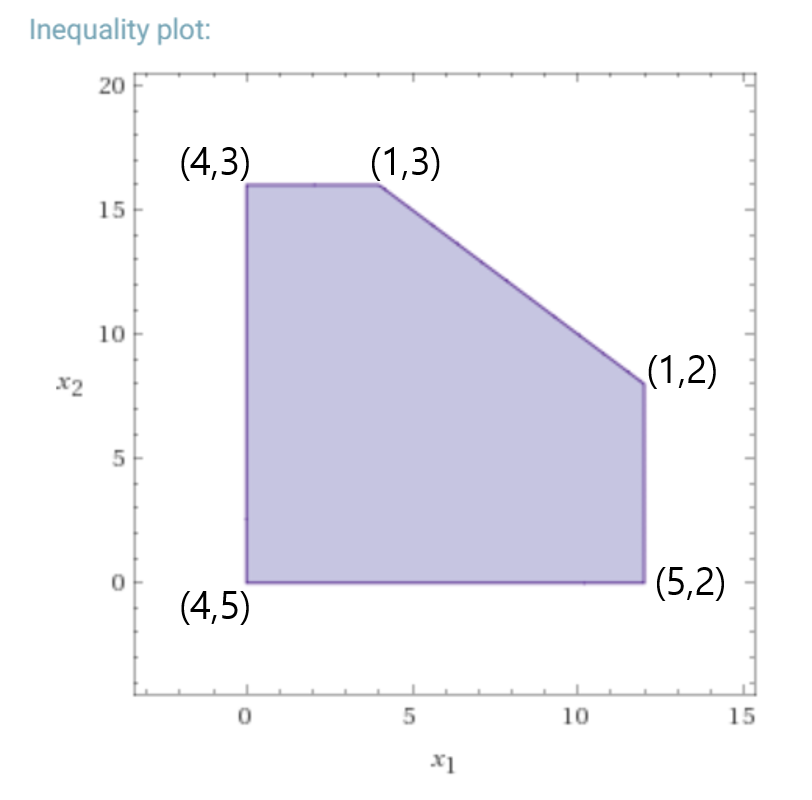
\includegraphics[scale=0.4]{figure1.png}
	\caption{Feasible Reigion}
\end{figure}

First, we are maximizing $18x_1 + 12.5x_2$. All coefficient is positive. So we loose constraint 4 and make constraing 2 tight. That lets us stop at $x_1 = 12$.
Then lets define $y_1 = 12 - x_1$ and $y_2 = x_2$. Then the objective function is $216-18y_1+12.5y_2$. $y_2$ coefficient is positive so we go on. The constraints are following

1 --- $-y_1 + y_2 \leq 8$

2 --- $y_1 \geq 0$

3 --- $y_2 \leq 16$

4 --- $y_1 \leq 12$

5 --- $y_2 \geq 0$

Lets make constraing 5 loose and 1 tight.
Then define $z_1 = y_1$ and $z_2 = 8 + y_1 -y_2$.
Then our objective function is $316 - 5.5z_1 - 12.5z_2$.
All coefficient is negative, so we stop here. This is the maximum point.The maximum is 316.

\item

The dual problem is following. If we multiply $y_i$ to each $i$thconstraint, we get the following.

$18x_1 + 12.5x_2 \leq 20y_1+12y_2+16y_3$ if $y_1,y_2,y_3,y_4,y_5 \geq 0, y_1+y_2-y_4 \geq 18, y_1 + y_3 - y_5 \geq 12.5$.
\\


So the new LP is 


min $20y_1+12y_2+16y_3$

and the constraints are

 $y_1,y_2,y_3,y_4,y_5 \geq 0, y_1+y_2-y_4 \geq 18, y_1 + y_3 - y_5 \geq 12.5$

This is minimized when $y_1 = 12.5$and $y_2 = 5.5$. The value is 316.
\end{enumerate}


\item 

Use memoization for solving this problem.

Make a array that has index $0$ to $V$.
I will store boolean values for each position of the array.
This value represents if the value(which is the index) is possible to make change. So for index $0$. The stored value is True.

Then from $1$ to $V$, we will look if it is possible to make change by looking at previous values.

For example if we are looking at index $k$, then we search for index $k-x_1$, $k-x_2$, ... $k-x_n$ . If one of those value is True, then the stored value for index $k$ is also True. Otherwise it is False.

My algorithm is correct, because in order to make value $k$ to be possible, it must have use one if the $x_1,x_2, ... x_n$. So looking previous values will make this algorithm correct.


\item

The majority element can exist at most two. My algorithm will give both if both exists.

Let's say that finding a majority element takes $T(n)$  time complexity for array length $n$. Then use divide and conquer algorithm and cut it in half.
For the left half, find the majority element. There could be two. Let's say they are $a$ and $b$. And for the right half, find the majority element. There could be two also. Let's say they are $c$ and $d$. For $a$ and $b$, look up the right half and count how many there is $a$ and $b$. That will take $O(n)$ time. Also for $c$ and $d$, look up the left half and count how many there is $c$ and $d$. This also will take $O(n)$. So If the sum of it is more than 1/3 of the total length, then it is one of the majority element.

The time complexity of this algorithm is $O(n\log n)$. It is because I cut the array in half. So, $T(n) = 2T(n/2) + O(n)$ and the master theorem tells that the time complexity is $O(n \log n)$




\end{enumerate}



\end{document}

\iffalse
\begin{figure}[hbt]
	\centering
	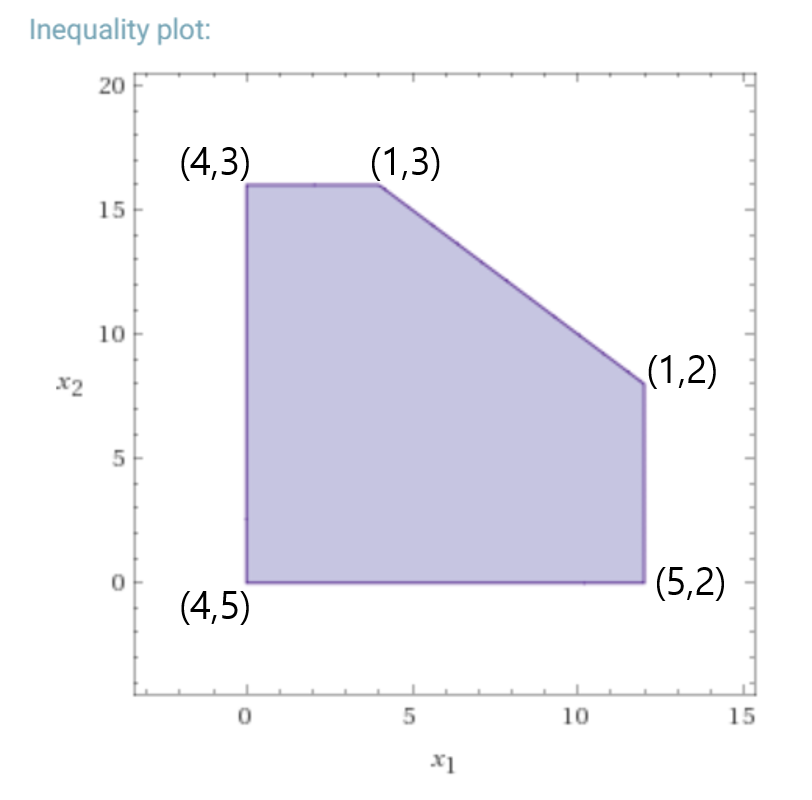
\includegraphics[scale=0.4]{figure1.png}
	\caption{Basic Tree}
\end{figure}
\fi
